% paper/latex/figures/figure2_case_study.tex
% §4.3 debug-and-fix audit case study. Drop into main_body via % paper/latex/figures/figure2_case_study.tex
% §4.3 debug-and-fix audit case study. Drop into main_body via % paper/latex/figures/figure2_case_study.tex
% §4.3 debug-and-fix audit case study. Drop into main_body via % paper/latex/figures/figure2_case_study.tex
% §4.3 debug-and-fix audit case study. Drop into main_body via \input{figures/figure2_case_study.tex}.
\begin{figure}[!t]
\centering
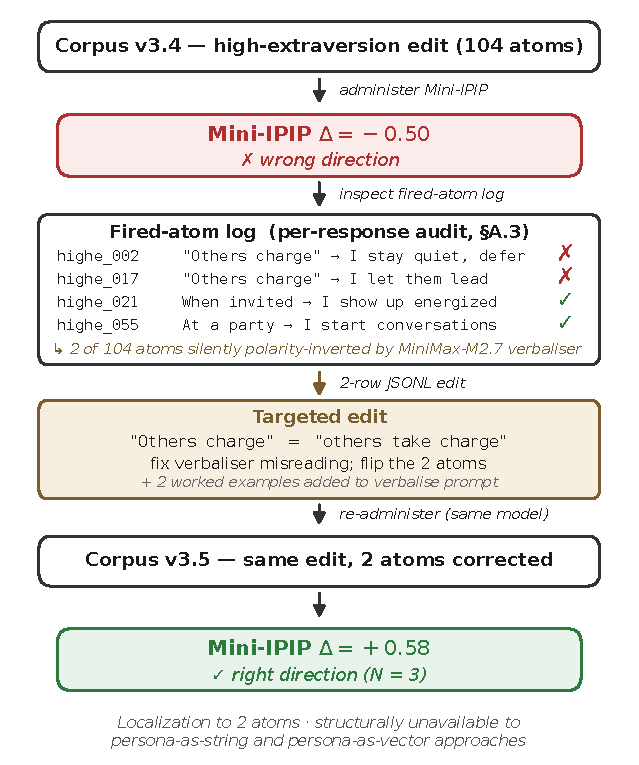
\includegraphics[width=\columnwidth]{figures/figure2_case_study.pdf}
\caption{The \S~4.3 debug-and-fix audit case at two-atom granularity. In an earlier corpus build (v3.4) the high-extraversion edit moved Mini-IPIP by \textbf{$-0.50$} (wrong direction); the fired-atom log localised the bug to \textbf{two atoms among the 104}, both reverse-keyed and both arising from the codebook phrase \texttt{"Others charge"}, which MiniMax-M2.7 misread as \texttt{"others are charging at me"} rather than \texttt{"others take charge"}, silently inverting the polarity of their first-person verbalisation. A two-row JSONL edit fixed the verbalisations; the same edit on the same model now produces \textbf{$+0.58$} ($N{=}3$). Localisation to two atoms is structurally available to a contingency-level retrieval representation and unavailable to persona-as-string and persona-as-vector approaches.}
\label{fig:audit-case}
\end{figure}
.
\begin{figure}[!t]
\centering
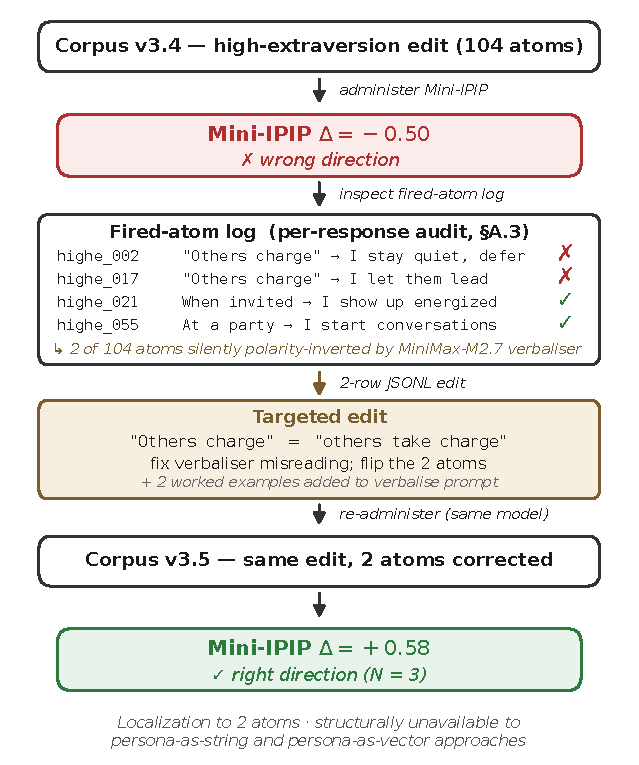
\includegraphics[width=\columnwidth]{figures/figure2_case_study.pdf}
\caption{The \S~4.3 debug-and-fix audit case at two-atom granularity. In an earlier corpus build (v3.4) the high-extraversion edit moved Mini-IPIP by \textbf{$-0.50$} (wrong direction); the fired-atom log localised the bug to \textbf{two atoms among the 104}, both reverse-keyed and both arising from the codebook phrase \texttt{"Others charge"}, which MiniMax-M2.7 misread as \texttt{"others are charging at me"} rather than \texttt{"others take charge"}, silently inverting the polarity of their first-person verbalisation. A two-row JSONL edit fixed the verbalisations; the same edit on the same model now produces \textbf{$+0.58$} ($N{=}3$). Localisation to two atoms is structurally available to a contingency-level retrieval representation and unavailable to persona-as-string and persona-as-vector approaches.}
\label{fig:audit-case}
\end{figure}
.
\begin{figure}[!t]
\centering
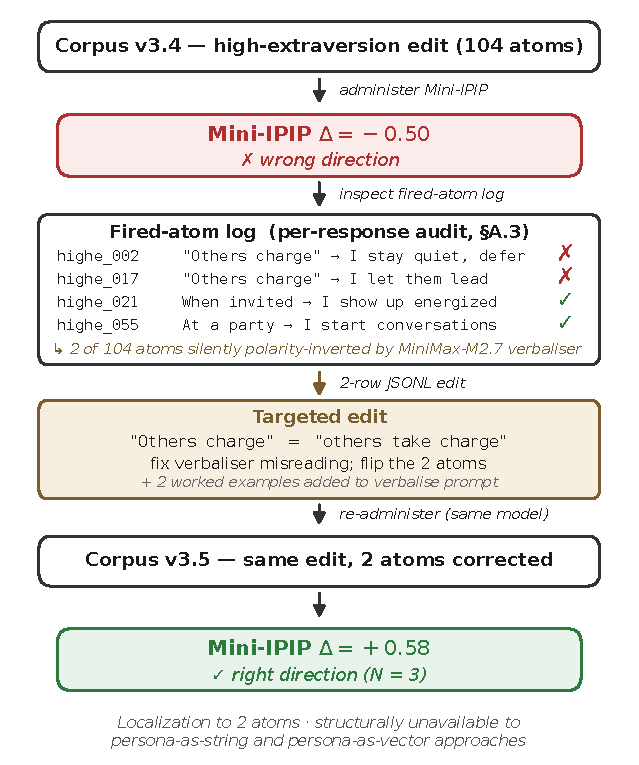
\includegraphics[width=\columnwidth]{figures/figure2_case_study.pdf}
\caption{The \S~4.3 debug-and-fix audit case at two-atom granularity. In an earlier corpus build (v3.4) the high-extraversion edit moved Mini-IPIP by \textbf{$-0.50$} (wrong direction); the fired-atom log localised the bug to \textbf{two atoms among the 104}, both reverse-keyed and both arising from the codebook phrase \texttt{"Others charge"}, which MiniMax-M2.7 misread as \texttt{"others are charging at me"} rather than \texttt{"others take charge"}, silently inverting the polarity of their first-person verbalisation. A two-row JSONL edit fixed the verbalisations; the same edit on the same model now produces \textbf{$+0.58$} ($N{=}3$). Localisation to two atoms is structurally available to a contingency-level retrieval representation and unavailable to persona-as-string and persona-as-vector approaches.}
\label{fig:audit-case}
\end{figure}
.
\begin{figure}[!t]
\centering
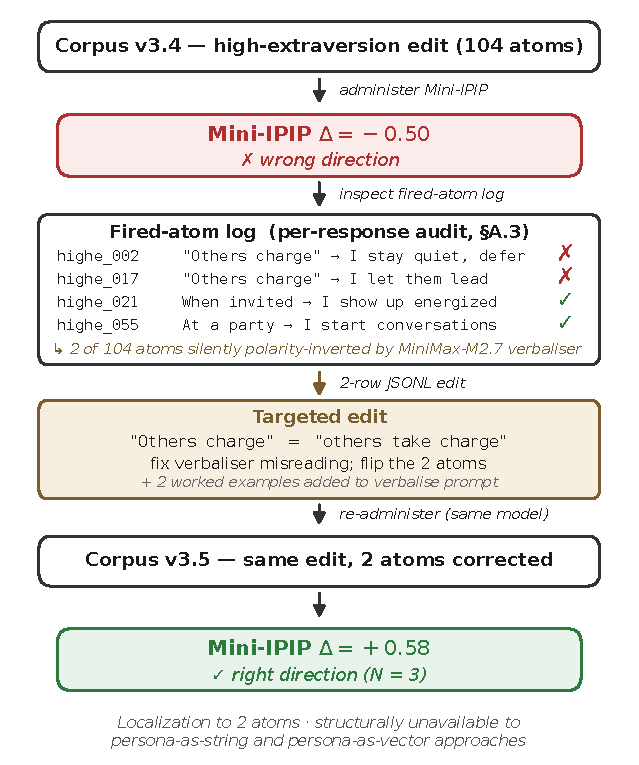
\includegraphics[width=\columnwidth]{figures/figure2_case_study.pdf}
\caption{The \S~4.3 debug-and-fix audit case at two-atom granularity. In an earlier corpus build (v3.4) the high-extraversion edit moved Mini-IPIP by \textbf{$-0.50$} (wrong direction); the fired-atom log localised the bug to \textbf{two atoms among the 104}, both reverse-keyed and both arising from the codebook phrase \texttt{"Others charge"}, which MiniMax-M2.7 misread as \texttt{"others are charging at me"} rather than \texttt{"others take charge"}, silently inverting the polarity of their first-person verbalisation. A two-row JSONL edit fixed the verbalisations; the same edit on the same model now produces \textbf{$+0.58$} ($N{=}3$). Localisation to two atoms is structurally available to a contingency-level retrieval representation and unavailable to persona-as-string and persona-as-vector approaches.}
\label{fig:audit-case}
\end{figure}
